
A continuous distribution  long tail and narrow while maintaing a constant mean. The gamma distribution fulfills these criteria.

Here we consider a slight modification to the traditional Gamma distribution in the form of a truncated version. Let $\alpha, \beta > 0$. A random variable $X$ follows the truncated gamma distribution $\Gamma^T(\alpha, \beta)$ if it has the probability density function 
%
\begin{align}
  f_{\alpha,\beta}(x) = \begin{cases} K_{\alpha, \beta}\,
\frac{1}{\beta^{\alpha}\Gamma(\alpha)}\, x^{\alpha-1}\,e^{-x/\beta} & 0 \leq x \leq 1 \\
0 & \text{otherwise}.
\end{cases}
\end{align}
%
Here the factor $K_{\alpha,\beta}$ is needed due to the truncation of the probability density function for $x>0$ to ensure that
\begin{align}
  \int f_{\alpha,\beta}(x) \,dx = 1. \label{eq:gd1}
\end{align}
The value of $K_{\alpha,\beta}$ is the inverse of the cumulative probability $x \leq 1$ of the untruncated gamma distribution,
\begin{align}
  K_{\alpha,\beta} = \left(\int_0^{1} \frac{1}{\beta^{\alpha}\Gamma(\alpha)}\, x^{\alpha-1}\,e^{-x/\beta} \, dx \right)^{-1}.
\end{align}
With this the equality~\eqref{eq:gd1} clearly holds. Consider then the above network model in which the connection probabilities $P_{ij}$ are $\Gamma^T(\alpha, \beta)$ distributed. As $K_{\alpha,\beta}$ is results hold. We note the following results for the overall connection probability $\mu$,

\begin{align}
 \mu = \E(P_{ij}) = K_{\alpha,\beta} \, \alpha \beta,
\end{align}
and the expected occurrence of bidirectional connections
\begin{align}
  \E(P_{ij}^2) = K_{\alpha,\beta}^2 \, (\alpha^2 \beta^2 + \alpha \beta^2).
\end{align}

The overrepresentation is then
\begin{align}
  \sigma & = \frac{\E(P_{ij}^2)}{\E(P_{ij})^2} =% \frac{\alpha^2 \beta^2}{\alpha^2 \beta^2} + \frac{\alpha \beta^2}{\alpha^2 \beta^2} =
  1 + \frac{1}{\alpha}.
\end{align}


\begin{figure}[h!]
\centering
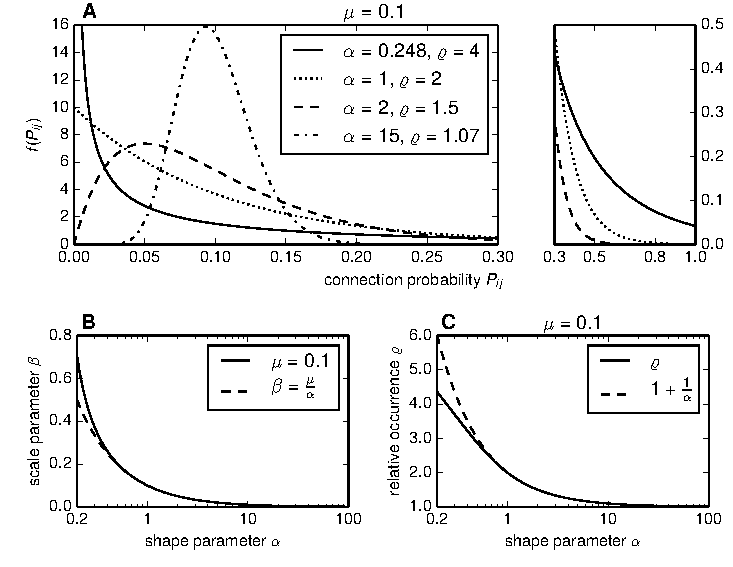
\includegraphics[width=\textwidth]{../lab/gamma_distribution/gamma_figure.png}
\caption{Probability density functions of the truncated gamma distribution for different shape parameters $\alpha$ and the induced relative overrepresentation of bidirectional connections $\sigma$ in the network. Note that only showing the distribution for values up to 0.5. For given $\alpha$ the parameter $\beta$ was estimated numerically to yield $\mu \approx 0.1$ in all distributions shown.}
\end{figure}


References: \href{http://herbsusmann.com/distributions/gamma-distribution-variance-proof.html}{Proof $\E(X^2)$}, 

